% !TeX spellcheck = sk_SK-Slovak
\documentclass[a4paper]{article}
\usepackage[slovak]{babel}
\usepackage[utf8]{inputenc}
\usepackage[T1]{fontenc}
\usepackage{a4wide}
\usepackage{amsmath}
\usepackage{amsfonts}
\usepackage{amssymb}
\usepackage{mathrsfs}
\usepackage[small,bf]{caption}
\usepackage{subcaption}
\usepackage{xcolor}
\usepackage{graphicx}
\usepackage{enumerate}
\usepackage{hyperref}
\usepackage{fancyvrb}
\usepackage{listings}
%\usepackage{lstautogobble}
\usepackage{stmaryrd}

\lstset{basicstyle=\ttfamily,
	mathescape=true,
	escapeinside=||%,
	%autogobble
}


\fvset{tabsize=4}


\pagestyle{empty}
\setlength{\parindent}{0pt}

\newenvironment{modenumerate}
{\enumerate\setupmodenumerate}
{\endenumerate}

\newif\ifmoditem
\newcommand{\setupmodenumerate}{%
	\global\moditemfalse
	\let\origmakelabel\makelabel
	\def\moditem##1{\global\moditemtrue\def\mesymbol{##1}\item}%
	\def\makelabel##1{%
		\origmakelabel{##1\ifmoditem\rlap{\mesymbol}\fi\enspace}%
		\global\moditemfalse}%
}

\makeatletter
\def\@seccntformat#1{%
	\expandafter\ifx\csname c@#1\endcsname\c@section\else
	\csname the#1\endcsname\quad
	\fi}
\makeatother

\begin{document} 
	
	\pagenumbering{arabic}
	\pagestyle{plain}
	
	\begin{center}
		\sc\large
		Neurónové siete\\
		Projekt 1\\
		Viacvrstvový klasifikátor 
	\end{center}
	
	Autor: Marián Kravec
	\\
	
	Našou úlohou je natrénovať viacvrstvovú neurónovú sieť ktorá dokáže zatriedi dvojrozmerné dáta do troch tried. Ide o supervised learning keďže naše trénovacie aj testovacie dáta sú oštítkované. 
	\\
	
	\section{Dáta}
	
	Máme dva datasety, trénovací dataset a testovací dataset. Trénovací dataset is rozdelíme v pomere 8:2 na estimačné a validačné dáta. Estimačné dáta použijeme na trénovanie modelu, validačné dáta použijeme na výber najlepšieho z pomedzi viacerých modelov a testovacie dáta použijeme na finálne určenie chyby a presnosti nášho výsledného modelu.
	\\
	
	Dáta si najskôr normalizujeme. Aby normalízacia totožná cez všetky datasety na normalizáciu použijeme iba estimačné dáta (o všetkých dát odčítame priemer estimačných dát aby sme ich vycentrovali, a vydelíme ich smerodajnou odchýlkou aby sme normalizovali ich rozptyl v jednotlivých smeroch). Na normalizáciu používame iba estimačné dáta aby sme zaručili, že výsledné normalizované dáta boli vždy porovnateľné. 
	
	\section{Architektúra}
	
	Na klasifikáciu použije trojvrstvovú neurónovú sieť (čiže neurónovú sieť s dvomi skrytými vrstvami). Na prvej skrytej vrstve použijeme aktivačnú vrstvu ReLU, druhá skrytá vrstva implementuje hyperbolický tangens and finálna výstupná vrstva využíva logistickú funkciu.
	\\
	
	Rýchlosť učenia je určená pomocou algoritmu Adam pričom ako parametre tohto algoritmu sme použili tieto hodnoty: $\alpha=0.1$, $\beta_1=0.9$, $\beta_2=0.99$. 
	\\
	
	Aby sme zaručili, že váhu nevyletia do vysokých čísel použijeme regularizáciu. Konkrétne použijeme implicitnú metódu weight decay s parametrom $\epsilon = 0.9995$, čiže nebudeme váhy ovplyvňovať príliš.
	\\
	
	Update váh je pomocou štandardného backpropagation algoritmu.
	\\
	
	Model je trénovaný batch metódou (všetky trénovacie vstupy sú použité naraz) pričom model je trénovaný na 500 epoch.
	\newpage
	
	\section{Optimalizované hyperparametre}
	
	Ako optimalizované hyperparametre sme si vybrali veľkosti (počty neurónov), samozrejme veľkosť vstupnej a výstupnej vrstvy je pevne daná vstupom a požadovaným výstupom, v našom prípade je táto veľkosť nasledovná, vstupná vrstva má veľkosť 2 a výstupná vrstva má veľkosť 3. Preto my budeme optimalizovať veľkosti dvoch skrytých vrstiev.
	\\
	
	Konkrétne vyskúšame všetky kombinácie veľkostí vrstiev medzi hodnotami 10 a 24 s krokom 2. Čiže 7 hodnôt pre každú vrstvu, dohromady 49 možností.
	\\
	
	Keď spustíme náš program dostaneme takéto hodnoty, trénovacích chýb, validačných chýb a časov trénovania:
	\\
	
	Trénovacie chyby jednotlivých modelov:
	\begin{table}[!h]
\begin{tabular}{|p{0.08\textwidth}|p{0.08\textwidth}|p{0.08\textwidth}|p{0.08\textwidth}|p{0.08\textwidth}|p{0.08\textwidth}|p{0.08\textwidth}|p{0.08\textwidth}|p{0.08\textwidth}|}
\hline
& 10& 12& 14& 16& 18& 20& 22& 24\\ \hline10 & 0.061& 0.186& 0.053& 0.037& 0.031& 0.028& 0.051& 0.038\\ \hline
12 & 0.104& 0.087& 0.036& 0.029& 0.03& 0.023& 0.023& 0.036\\ \hline
14 & 0.051& 0.061& 0.063& 0.038& 0.103& 0.026& 0.043& 0.024\\ \hline
16 & 0.029& 0.118& 0.047& 0.041& 0.07& 0.035& 0.052& 0.026\\ \hline
18 & 0.044& 0.032& 0.033& 0.027& 0.028& 0.038& 0.024& 0.029\\ \hline
20 & 0.085& 0.029& 0.025& 0.042& 0.033& 0.03& 0.025& 0.023\\ \hline
22 & 0.032& 0.041& 0.025& 0.03& 0.037& 0.026& 0.181& 0.052\\ \hline
24 & 0.067& 0.026& 0.025& 0.03& 0.023& 0.027& 0.03& 0.025\\ \hline
\end{tabular}
\end{table}


	Validačné chyby jednotlivých modelov
	\begin{table}[!h]
\begin{tabular}{|p{0.08\textwidth}|p{0.08\textwidth}|p{0.08\textwidth}|p{0.08\textwidth}|p{0.08\textwidth}|p{0.08\textwidth}|p{0.08\textwidth}|p{0.08\textwidth}|p{0.08\textwidth}|}
\hline
& 10& 12& 14& 16& 18& 20& 22& 24\\ \hline10 & 0.089& 0.209& 0.091& 0.041& 0.06& 0.048& 0.071& 0.049\\ \hline
12 & 0.139& 0.125& 0.058& 0.049& 0.05& 0.037& 0.038& 0.057\\ \hline
14 & 0.066& 0.094& 0.101& 0.054& 0.157& 0.037& 0.062& 0.037\\ \hline
16 & 0.038& 0.151& 0.07& 0.051& 0.115& 0.051& 0.078& 0.037\\ \hline
18 & 0.064& 0.041& 0.049& 0.037& 0.039& 0.047& 0.037& 0.058\\ \hline
20 & 0.104& 0.04& 0.037& 0.071& 0.05& 0.045& 0.039& 0.038\\ \hline
22 & 0.046& 0.074& 0.038& 0.056& 0.049& 0.035& 0.16& 0.08\\ \hline
24 & 0.085& 0.037& 0.037& 0.047& 0.03& 0.041& 0.04& 0.038\\ \hline
\end{tabular}
\end{table}

	
	Vidíme, že validačné chyby sú veľmi blízke trénovacím, čo nasväčšuje tomu, že asi nedochádza k pretrénovaniu modelu. V prípade časov trénovania vidíme, že zo zväčšujúcou sa veľkosťou vrstiev sa trénovací čas zväčšuje.
	\\
	\newpage
	Pre lepšiu vizualizáciu zobrazenie validačných chýb vo forme heatmapy.
	\begin{figure}[!h]
		\centering
		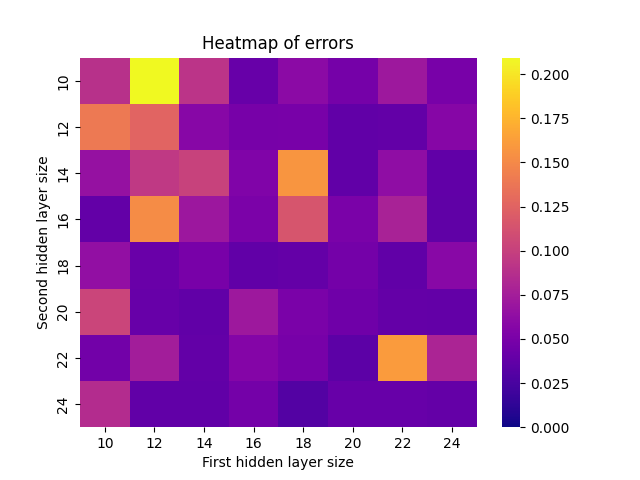
\includegraphics[width=0.77\textwidth]{../heatmap_errors.png}
		\caption{Heatmapa validačných chýb modelov pre rôzne veľkosti skrytých vrstiev}
	\end{figure}

	\begin{figure}[!h]
		\centering
		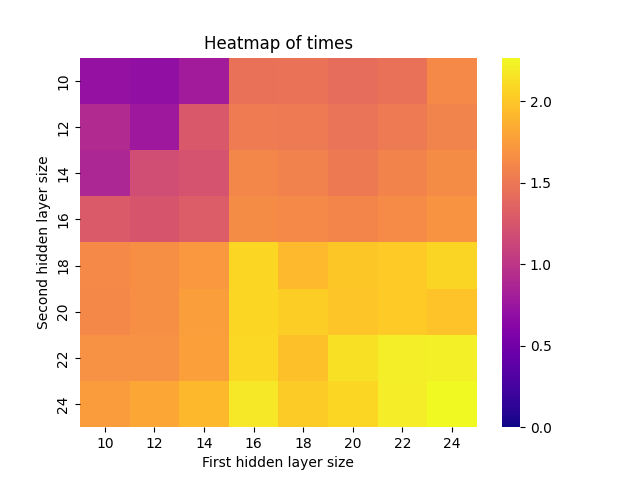
\includegraphics[width=0.77\textwidth]{../heatmap_time.png}
		\caption{Heatmapa časov trénovania modelov pre rôzne veľkosti skrytých vrstiev}
	\end{figure}

	Vidíme, že najlepšiu validačnú chybu máme pre prvú skrytú vrstvu veľkosti 18 a druhú skrytú vrstvu veľkosti 24. Preto náš finálny model budeme trénovať s vrstvami práve tejto veľkosti. Tento model budeme trénovať na celom trénovacom datasete (estimačný aj validačný) a na určenie kvality modelu použijeme testovacie dáta.
	\\
	
	\begin{figure}[!h]
		\centering
		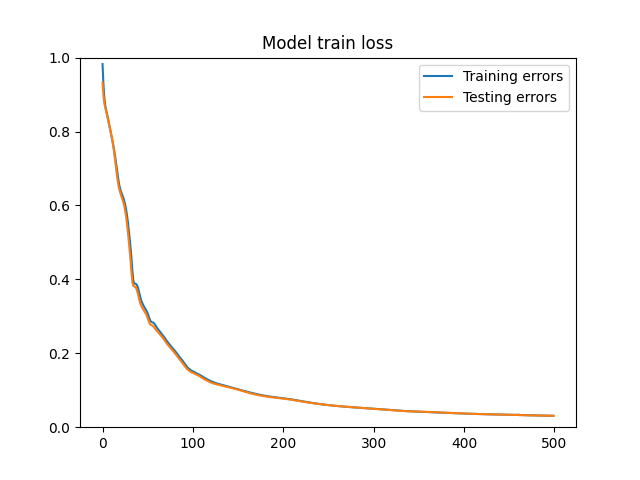
\includegraphics[width=\textwidth]{../errors.png}
		\caption{Priebeh trénovacej a testovacej chyby počas trénovania modelu }
	\end{figure}
	 
	Vídíme, že sa počas trénovania postupne znižovala trénovacia chyba, prekvapivo, testovacia chyba ju po celý čas takmer dokonale kopíruje, čo nám hovorí, že model nie je pretrénovaný (inak by ku koncu začínala testovacia chyba rásť). Zároveň vidíme, že výsledná chyba vyzerá byť pomerne nízka. Aby sme dostali lepšiu predstavu o tom ako dobre náš model rozoznáva jednotlivé triedy, na to použijeme confusion matrix.
	
	\begin{table}[!h]
\begin{tabular}{|p{0.08\textwidth}|p{0.08\textwidth}|p{0.08\textwidth}|p{0.08\textwidth}|}
\hline
& A& C& B\\ \hline
A & 97.18\% & 2.46\% & 0.35\% \\ \hline
C & 0.0\% & 99.54\% & 0.46\% \\ \hline
B & 0.16\% & 1.59\% & 98.25\% \\ \hline
\end{tabular}
\end{table}

	
	Vidíme, že vo všetkých kategóriách je náš model presný na viac ako 95\%. Nakoniec si ešte tento výsledok vizualizujeme. Keďže ide o dvojrozmerné dáta použijeme klasický scatter plot, pričom veľkými bodmi budeme reprezentovať skutočné hodnoty tried a malými bodkami triedy pridelené naším modelom, pri takejto vizualizácii ak sa náš model netrafil do skutočnej triedy uvidíme malú bodku v strede väčšej bodky inej farby.
	\newpage
	\begin{figure}[!h]
		\centering
		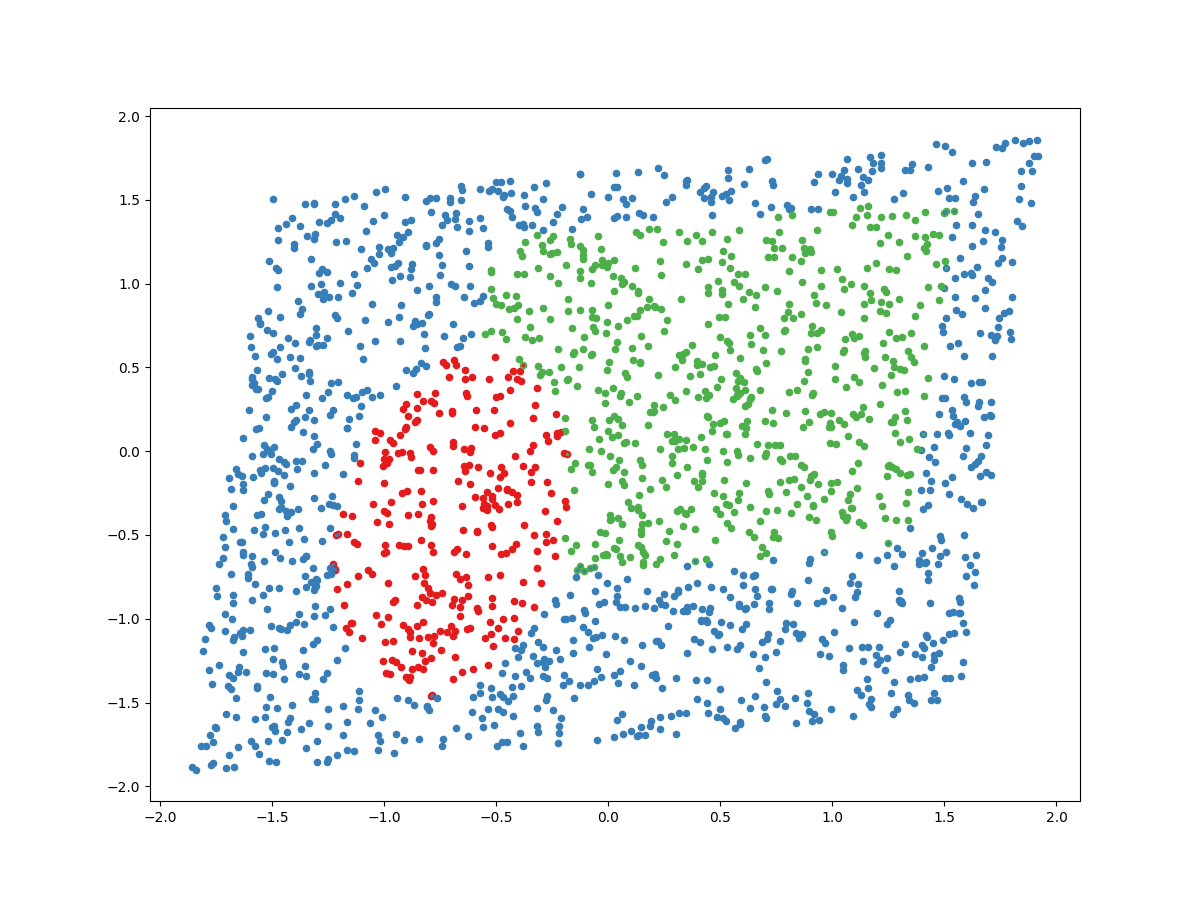
\includegraphics[width=\textwidth]{../decision_model.png}
		\caption{Vizualizácia skutočných a modelom pridelených tried pre testovacie dáta}
	\end{figure}
	
	Vidíme, že drvivá väčšina bodov je zatriedená správne, niekoľko nesprávne zatriedených bodov sa nachádza na hraniciach medzi kategóriami.
	
\end{document}